\section{讨论:连接数可扩放性}
\label{socksdirect:sec:discussion}


使用商用 RDMA 网卡时,\sys {} 对大量连接的可伸缩性受底层传输层(即共享内存和RDMA)的限制。
为了表明 \libipc {} 和管程不是瓶颈,本节在两个重用RDMA QP和共享内存的进程之间创建了很多连接。使用 \libipc {} 的应用程序线程每秒可以创建1.4~M个新连接,这是Linux的20倍和mTCP的2倍 \cite {jeong2014mtcp}。管程每秒可以创建5.3~M个连接。

由于主机内的进程数量有限,因此共享内存连接的数量可能不会很大。
但是,一台主机可能连接到许多其他主机,RDMA的可扩展性成为一个问题。
RDMA 的可扩展性归结为两个问题。
首先,RDMA 网卡使用网卡内存作为缓存来保持每个连接状态。当有数千个并发连接时,性能受到频繁缓存未命中的影响 \cite {mprdma,kaminsky2016design,kalia2018datacenter}。
因为 RDMA 传统上部署在中小型集群中,传统 RDMA 网卡上的内存容量较小。
随着近年来大规模的 RDMA 部署 \cite {guo2016rdma},大多数网卡厂商已经意识到这个问题。
因此,近期的商用网卡内存容量越来越大,例如 Mellanox ConnectX-5~\cite{connectx-5},可以存储上千条连接的状态 \cite {kalia2018datacenter}。而本文使用的可编程网卡甚至拥有数千兆字节的DRAM~ \cite {mellanox-innova,mellanox-bluefield,smartnic}。
因此,本文预测未来的数据中心不会为网卡缓存未命中问题担心过多。下一节将基于可编程网卡,提出一个连接数可扩放的传输层实现框架。
第二个问题是本文的测试平台中建立RDMA连接需要大约 $30 \mu s$,这对于短连接很重要。此过程仅涉及本地CPU和网卡之间的通信,因此这个连接建立延迟是可以优化的。

在大量并发连接下的服务质量保证(Quality of Service,QoS)也是数据中心的重要需求。
传统网络协议栈在操作系统内核实现服务质量保证。
而对于本章使用的硬件传输协议,将数据平面性能隔离和拥塞控制卸载到 RDMA 网卡上是一个越来越流行的研究方向 \cite {peter2016arrakis,zhu2015congestion,lu2017memory,mprdma,mittal2018revisiting},因为数据中心的网卡正变得越来越可编程  \cite{smartnic,cavium,kaufmann2015flexnic,mellanox-innova,mellanox-bluefield},而且公有云已经在虚拟机之外的网络功能中提供了 QoS \cite {li2016clicknp,panda2016netbricks,floem-osdi18}。

连接数可扩放性需要存储每个连接的传输层和数据包缓冲区。针对传输层状态问题,接下来的两节提出两种方案:在可编程网卡中或主机 CPU 的用户态库中存储连接状态并实现传输层处理。针对数据包缓冲区问题,最后一节提出多套接字共享队列,将两个进程间多个连接的缓冲区合并。

\subsection{基于可编程网卡的传输层}
\label{socksdirect:sec:smartnic}

%\textbf{Communicating with TCP/IP peers.}
%We use a user-space networking stack to communicate with regular TCP/IP peers, but the compatibility may be limited~\cite{yasukata2016stackmap}.
%To solve this problem, after receiving the TCP SYN+ACK, the monitor can create an established kernel TCP connection using TCP connection repair~\cite{tcp-connection-repair}.
%Moreover, if the application and monitor share a network namespace, the monitor can send the kernel 文件描述符 to the application via Unix domain socket, then \libipc{} can use the 文件描述符 without delegation to the monitor.

%\textbf{Connecting to many RDMA capable hosts.}
%With a lot of hosts, the 网卡 still suffer from performance degradation due to large number of connections.
%In contrast, user-space networking stack alleviates this problem because the 网卡 is stateless.
%We provide a socket option to enable applications to delegate operations to the monitor and use user-space networking stack even if the peer supports RDMA.
%An application can choose to use RDMA for latency sensitive and throughput demanding connections, and user-space networking stack for others.






本节基于可编程网卡和第 \ref{chapter:socksdirect} 章的网络数据包处理平台和第 \ref{chapter:kvdirect} 章的内存键值存储,实现了一个连接数可扩放的 RDMA 网卡。
实现连接数可扩放的主要挑战是在缓存不命中率很高时,高吞吐量地存取主机内存中的连接状态,并能隐藏存取延迟。这正是第 \ref{chapter:kvdirect} 章所解决的问题,因此本节基于高性能键值存储实现了可扩放的连接状态存储。


\begin{figure}[htbp]
	\centering
	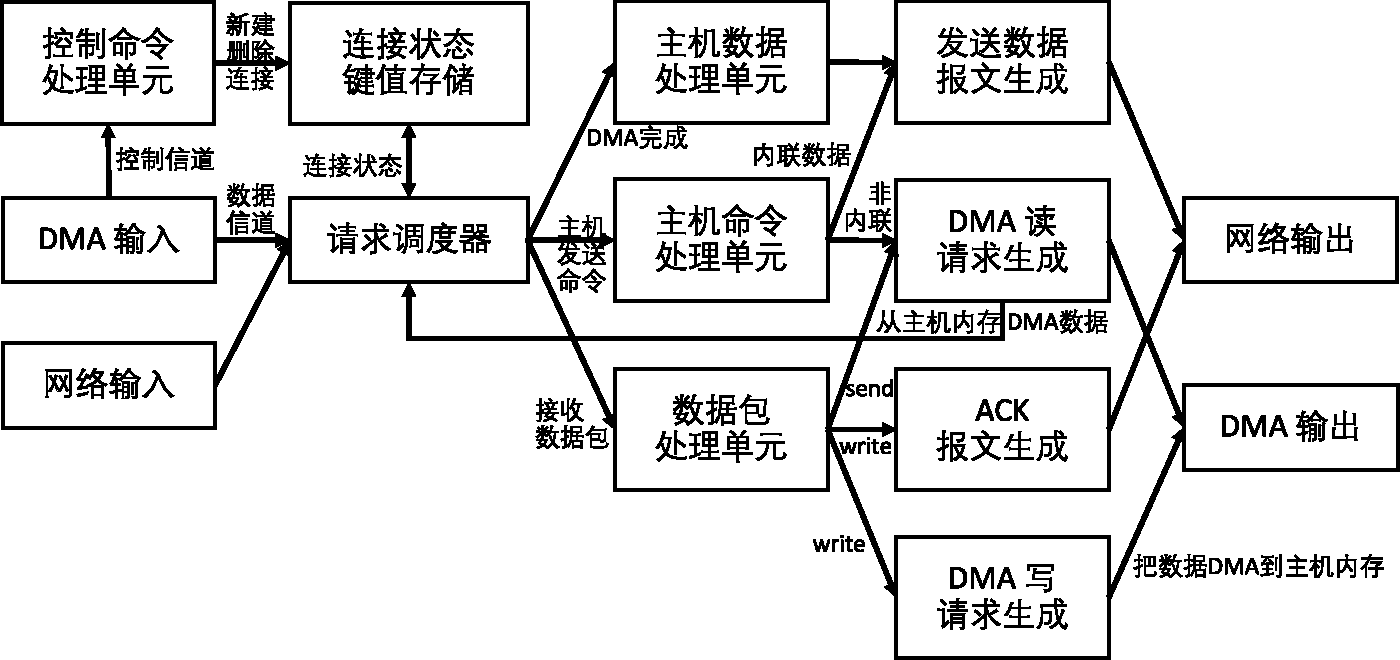
\includegraphics[width=1.0\textwidth]{images/scalable_rdma.pdf}	
	\caption{基于可编程网卡的连接数可扩放 RDMA。}
	\label{socksdirect:fig:scalable-rdma}
\end{figure}

基于可编程网卡的 RDMA 网卡架构如图 \ref{socksdirect:fig:scalable-rdma} 所示。
RDMA 网卡需要处理来自主机的控制和数据传输命令(工作请求,work request),还需要处理来自网络的数据包。
对于控制和数据传输命令,主机 CPU 把工作请求放入主机内存中的工作队列(work queue),再通过 PCIe DMA 发送到网卡 \cite{kalia2016design}。
通过网络接口接收的数据包也被放入网卡的输入缓冲区,对应工作队列中的一个工作请求。
请求调度器根据数据包的五元组(five-tuple)信息或主机命令中的连接编号,从连接状态键值存储中取出连接的状态信息,并按照连接的优先级,将工作请求和当前连接状态分类放入网卡内部的不同工作队列。
由于 RDMA 消息的处理是有状态的,处理同一个连接的两个相邻数据包可能存在依赖关系。为此,请求调度器记录正在处理的连接,并只调度未被处理连接的工作请求,这与第 \ref{chapter:kvdirect} 章键值存储中同一个键的消息处理方式相同。
对于接收到的数据包,接收处理单元按照 RDMA 消息的类型处理。对于 RDMA 单边写(write)消息,只需生成主机 DMA 操作,将数据写入主机内存的相应位置,并回复 ACK 消息。对于 RDMA 单边读(read)、原子(atomic)和双边发送(send)消息,需要从主机内存中读取相应的数据,才能进行下一步操作。为了隐藏主机内存读取的 DMA 延迟,生成主机内存的 DMA 读请求后,还需要生成一个新的工作请求,等待 DMA 完成后再进行下一步处理。
这种新工作请求被送回请求调度器,同时标记等待条件。
当 DMA 完成后,请求调度器将处理这个新工作请求,发送数据到网络或将数据 DMA 到主机内存。
数据发送命令 send 的处理方式与 RDMA 单边读(read)消息的处理方式类似。
数据接收命令 recv 不需要网卡主动处理,而是从网络收到双边发送(send)或带立即数的单边写(write with immediate)消息时,才需要匹配对应的 recv 工作请求。

上述处理流程的性能挑战是单个时钟周期内很难完成一个工作请求的有状态处理(如拥塞控制),而同一个连接的工作请求不能并行处理,从而降低了单连接吞吐量。解决方案是将工作请求的处理流水线(pipeline)化,每个流水级(stage)处理连接状态的不同部分,因此流水级之间没有数据依赖。在每个流水级内设置第 \ref{chapter:kvdirect} 章的数据转发(data forwarding)机制,使尚未写回请求调度器的状态更新对后续的工作请求可见。这样,同一个连接有依赖关系的多个工作请求可以在不同的流水级间并发处理。对于这类可以通过流水线和数据转发解决的依赖,请求调度器就不必记录依赖关系,而是认为所有此类请求都是不相关的。


\subsection{基于 CPU 的传输层}
\label{socksdirect:subsec:cpu-transport}

实现连接数可扩放性的另一种方案是在主机 CPU 上实现传输层协议,从而网卡无需为每个连接存储状态,只需实现无状态卸载。
网卡无状态卸载的常见方案是用户态协议栈与网卡之间使用收发数据包接口,而非 RDMA 远程内存访问接口。
基于数据包的实现除了可以处理大量并发连接,还可以在不支持 RDMA 的虚拟化平台上使用。例如,微软 Azure 云的很多虚拟机实例不支持 RDMA,但支持 DPDK 和 LibVMA 等高性能数据包接口,基于数据包的传输层将可以在这些虚拟化平台上使用。

LibVMA 与网卡之间使用高性能数据包收发接口。LibVMA 的兼容性、性能和多核可扩放性问题主要是由于其 VFS 层。因此,本节利用 LibVMA 实现传输层功能和网卡接口,替换 \libipc{} 中的环形缓冲区和 RDMA 硬件传输层。
LibVMA \cite{libvma} 用户态套接字库的结构与图 \ref{socksdirect:fig:libsd-architecture} 的 \libipc{} 库类似,都是由 API 封装、VFS 层、队列层和传输层构成。
LibVMA 的队列层和传输层由 LwIP 轻量级 TCP/IP 协议栈和 Mellnox 网卡的高速数据包收发接口组成。
为了使用 LibVMA,在 \libipc{} 中将基于环形缓冲区的队列替换成 LwIP 的发送接收接口。
测试表明,LibVMA 中的 LwIP 和网卡接口部分发送和接收小数据包的吞吐量为 18 M 次每秒;\libipc{} 中的 API 封装和 VFS 层的吞吐量为 27 M 次每秒。这意味着基于 LibVMA 的 \libipc{} 吞吐量大约可达 10.8M 个小数据包每秒。

为了实现基于 TCP/IP 的零拷贝,LibVMA 中的 LwIP 传输层需要修改。
为了页面重映射,发送和接收的有效载荷需要对齐到 4~KiB 边界。
发送时,\libipc{} 组建一个两块缓冲区构成的数据包:首先是从数据包头模板经过 LwIP 传输层组建的数据包头部,然后是零拷贝的有效载荷。
\libipc{} 利用网卡的分散-聚集(scatter-gather)支持来让网卡把两块缓冲区组成一个数据包。
接收时,\libipc{} 使用一个包含两块缓冲区的接收工作请求,首先是恰好能容纳标准 TCP/IP 数据包头的 54 字节缓冲区,然后是页面对齐的有效载荷缓冲区。
与第 \ref{socksdirect:subsec:lockless-queue} 章的设计相同,\libipc{} 在接收到数据包后及时补充 \texttt{recv} 工作请求,保持网卡始终有接收缓冲区可用。


上述基于数据包接口的方案需要 LibVMA 库为每条连接插入一条流重定向(flow steering)规则,把接收到的数据包映射到接收工作队列。这仍然需要网卡为每条连接维护状态,因此如第 \ref{socksdirect:sec:evaluation} 节的评估结果显示的,并发连接数较多时性能仍然会下降。
为了让网卡完全不保存连接状态,可以用可编程网卡实现不可靠、无拥塞控制的单边 RDMA 写操作(目前 Mellanox RDMA 网卡不支持基于不可靠数据报的单边 RDMA)。
单边 RDMA 写操作中包含远程主机上的内存地址,因此接收端网卡只需将有效载荷通过 PCIe DMA 写入数据包中指定的地址。
这样就可以应用本章第 \ref{socksdirect:subsec:lockless-queue} 节的环形缓冲区设计,发送端通过不可靠信道将环形缓冲区的变化同步到接收端。
启用了 RDMA 的数据中心网络丢包率很低,因此可以通过超时检测丢包。具体地,接收端发现环形缓冲区内有数据后即发送确认(ACK)包;发送端如果超时未收到确认包则重传。
为了实现基于窗口的拥塞控制,发送端需要为每个环形缓冲区(即每条连接)维护一个发送窗口,并在收到确认包和显式拥塞通知(ECN)时调整发送窗口。
丢包恢复和拥塞控制等传输层功能增加的 CPU 开销是有限的。
通过这种方法可以解决网卡连接数的可扩放性问题。


\subsection{多套接字共享队列}
\label{socksdirect:subsec:multiplex-conn}

很多应用在两个进程间建立多个套接字连接。例如,数据库的多个客户端线程和多个服务器线程之间可能两两建立连接。HTTP 负载均衡器与后端 Web 服务之间往往为每个 HTTP 请求建立一个连接。一些其他的传输层协议(如 SCTP)和应用层协议(如 QUIC 和很多 RPC 库)也提供多连接的抽象。在传统设计中,每个连接需要独立的缓冲区,因而所需的缓冲区数量较多。

为了降低内存占用,提升内存访问的局部性,如图 \ref{socksdirect:fig:fork-rdwr},本文使用一条队列来共享一对线程之间的所有连接。队列中的每个数据元素用其文件描述符标识。通过使用一条队列,可以降低每套接字的内存占用、随机内存访问和缓存不命中。



\begin{figure}[htbp]
	\centering
	\subfloat[传统队列结构。]{
		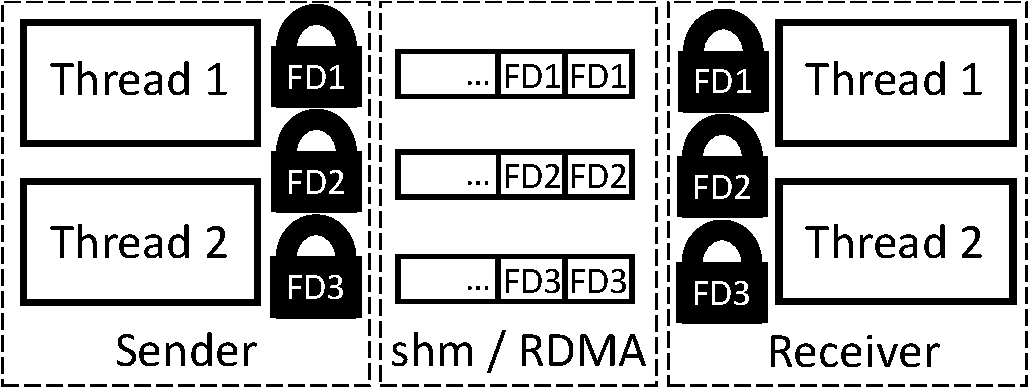
\includegraphics[width=0.6\textwidth]{images/fork_linux}
	}

	\subfloat[多套接字共享队列结构。]{
		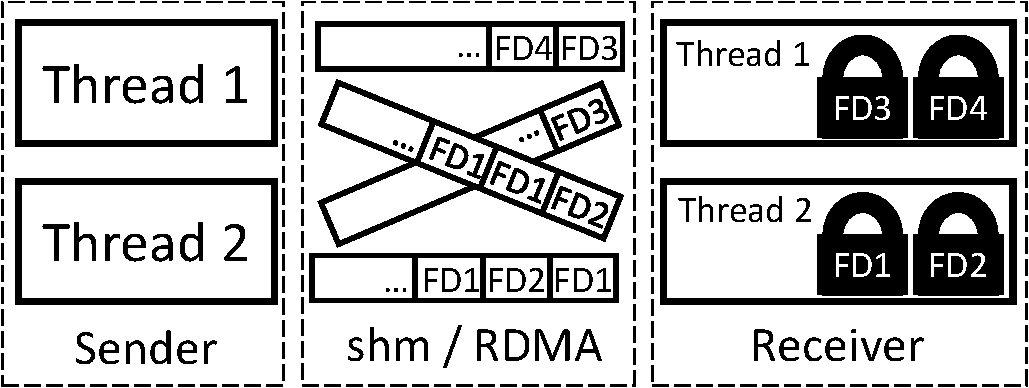
\includegraphics[width=0.6\textwidth]{images/fork_rdwr}
	}
	\caption{队列结构的比较。假设发送方和接收方各有两个线程。 首先,在每对发送方和接收方线程之间创建对等队列。不是用锁来保护队列,而是将每个文件描述符指定给接收方线程以确保排序。其次,来自所有连接(文件描述符)的数据通过共享队列进行多路复用,而不是每个文件描述符一个队列。}
	\label{socksdirect:fig:fork-rdwr}
\end{figure}

\iffalse
\begin{figure}[htbp]
	\centering
	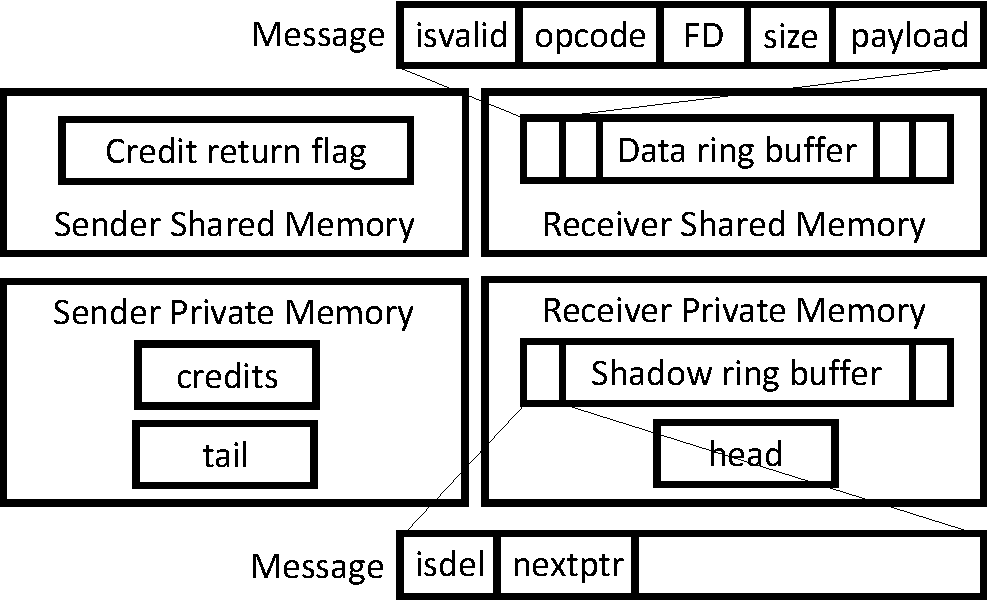
\includegraphics[width=0.8\textwidth]{images/locklessq_new}
	
	\caption{The structure of an inter-process queue.}
	
	\label{socksdirect:fig:locklessq-structure}
\end{figure}
\fi

\textbf{队列中的消息格式。}
在第 \ref{socksdirect:subsec:lockless-queue} 节的传统队列结构基础上,为每条消息在头部增加一个文件描述符域,表示接收端的文件描述符。这样,不同文件描述符的消息就可以共享一个队列。每条消息头部还增加一个 \textit{下一消息指针} 域,用于下述的事件轮询;增加一个 \textit{删除} 位,用于下述的从队列中间取消息。


\textbf{事件轮询。}
为每个 epoll 文件描述符集合维护一个位图。
当调用 \texttt{epoll\_wait} 时,轮流扫描所有的数据队列,并在位图中检查每个数据消息的文件描述符。
如果文件描述符在位图中,就返回给应用程序一个事件。
维护一个全局指针,以便从上次扫描的队列位置恢复数据队列的扫描。
为了避免多次扫描同一个消息,每条队列设置一个指针,保存上次扫描的位置。
由于应用程序可能在一个文件描述符上反复执行接收操作,直到该文件描述符的队列为空,本文一边扫描,一边为每个文件描述符创建一个消息链表,以加速重复的接收操作。
每个文件描述符维护两个指针,即该文件描述符的第一个和最后一个扫描过但尚未被接收走的消息。
当扫描文件描述符的一条新消息时,消息头部的下一消息指针域被更新,指向新扫描的消息,这就组成了同一文件描述符的消息链表。

\textbf{从队列中间取消息。}
为了从任意的文件描述符接收数据,队列需要支持从中间取走一条消息。
幸运的是,这并不经常发生。事件驱动的应用程序通常按照先到先处理的顺序处理到来的事件。
对于电平触发模式的 \texttt{epoll\_wait} 操作,\libipc{} 在队列中扫描所有消息,并返回那些文件描述符已被注册在 epoll 文件描述符集合中的消息。
因此,当应用程序调用 \texttt{recv} 时,取走的通常是队列头部的消息。

为了从队列的中间寻找特定文件描述符的消息,如果文件描述符的消息链表非空,则链表头就是要找的消息;如果为空,则需要在队列中遍历消息,从环形缓冲区的头指针遍历到未被分配的空间(用 \textit{有效} 位标识)。因此,当从队列中间取走一条消息时,其 \textit{有效} 位不能被清空。因此,每条消息增加一个 \textit{删除} 位。当消息从中间被取走时,该 \textit{删除} 位被设置。

\textbf{碎片整理。}
如果应用程序一直不接收某个文件描述符的数据,队列的空闲空间将变得碎片化。
当环形缓冲区中没有可用空间时,有可能其中仍有很多已被删除的消息,但因其位于未被接收的其他文件描述符消息之间,这些消息的空间无法被利用。
当环形缓冲区没有可用空间时,发送端通过共享内存中的控制寄存器,通知接收端进行碎片整理。
接收端扫描环形缓冲区中的可用空间,将尚未被接收的消息集中在一起,并将空闲空间返回给发送端。

%\textbf{Emergency queue.}
%Control messages may need to be delivered out-of-band when the queue is full. For example, in order to close the receive direction while sending data, the shutdown message should not be blocked by unconsumed data in the queue. To this end, we add an \textit{emergency queue} alongside each data queue.
%A receiver will always retrieve messages in the emergency queue immediately.


%\subsubsection{Zero Copy TCP}
%\label{socksdirect:subsec:zero-copy-tcp}
%


下面评估多套接字共享队列的连接数可扩放性。
测试前在两个进程间预先建立指定数量的连接,然后轮流(round-robin)使用这些连接以乒乓(ping-pong)的模式收发数据。
图 \ref{socksdirect:fig:eval-connnum-tput} 显示了不同并发连接数量下的单核吞吐量。
\sys{} 可以用 16 GB 的主机内存支持 100 M 条并发连接,并且在如此高的并发度下吞吐量不降低。
作为对比,RDMA、LibVMA 和 Linux 的性能随连接数量的增加而迅速降低。
对于 RDMA,性能在超过 512 条并发连接后迅速降低,这是由于 RDMA 传输层状态占满了网卡缓冲区。
尽管 LibVMA 和 Linux 并不使用 RDMA 作为传输层,它们为每条连接维护缓冲区,因此在数千条并发连接时会导致 CPU 缓存和 TLB 不命中。
此外,LibVMA 在网卡中为每个连接安装了一条连接重定向规则(flow steering rule),这也会导致网卡缓存不命中。

\begin{figure}[htbp]
	\centering
	\subfloat[单机内吞吐量。]{                    
		%\begin{minipage}{0.4\textwidth}
		\centering
		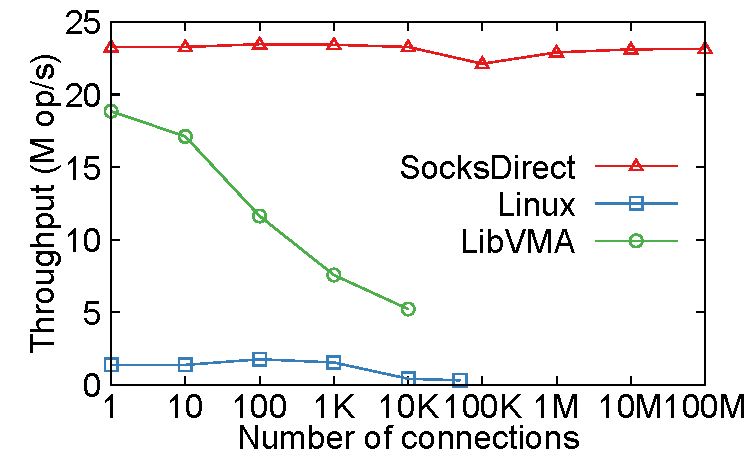
\includegraphics[width=0.5\textwidth]{eval/microbenchmark/connnum-ipc-tput.pdf}
		\label{socksdirect:fig:eval-connnum-ipc-tput}
		%\end{minipage}
	}
	\subfloat[跨主机吞吐量。]{
		%\begin{minipage}{0.4\textwidth}
		\centering 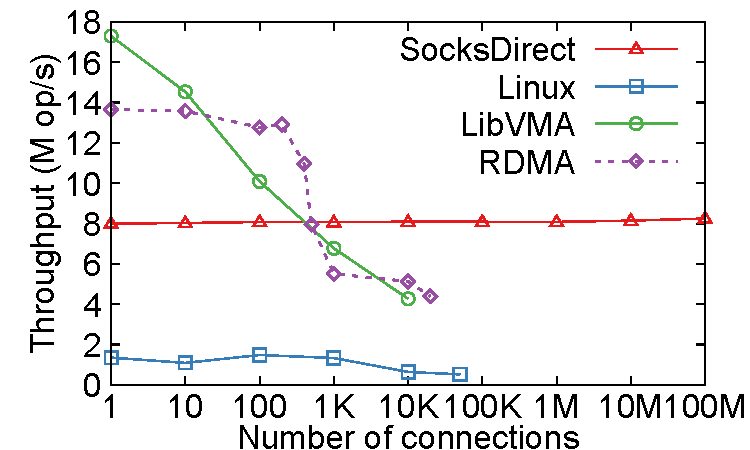
\includegraphics[width=0.5\textwidth]{eval/microbenchmark/connnum-network-tput.pdf}
		\label{socksdirect:fig:eval-connnum-network-tput}
		%\end{minipage}
	}
	
	\caption{不同并发连接数量下的单核吞吐量。}
	\label{socksdirect:fig:eval-connnum-tput}
\end{figure}


\section{局限性与讨论}
\label{sockdirect:sec:limitation}

除了 \S\ref{socksdirect:sec:discussion} 讨论的高并发下的性能局限,本章将讨论 \sys{} 在兼容性和 CPU 开销方面的局限性,以及协议栈的接口抽象。

\subsection{兼容性局限}



\parab{传输层。}
\sys{} 把传输层机制卸载到 RDMA 网卡。读者可能对 RDMA 网卡的传输层机制有一些疑问。例如,大多数商用网卡依赖于基于优先级的流控(PFC)来消除以太网上由于拥塞导致的丢包。PFC 会带来很多问题,诸如线头阻塞,拥塞扩散,甚至死锁 \cite{guo2016rdma},使网络难以管理和理解。我们注意到很多旨在提高 RDMA 传输层性能的工作。近年来提出的 RDMA 拥塞控制算法 \cite{zhu2015congestion,mprdma,mittal2015timely,hpcc} 不仅改进了吞吐量和延迟,还减少了 PFC 暂停(pause)帧的数量。很多高级丢包恢复机制 \cite{mittal2018revisiting,lu2017memory} 也使 RDMA 在有丢包的网络上不再需要 PFC。因此,我们预期未来的 RDMA 网卡可以在有丢包的数据中心网络上提供低延迟和高吞吐量的传输层。

\parab{优先级与服务质量保证。}
多个线程共享同一 CPU 核心时,\sys{} 使用非抢占调度。但是,为了保证实时性和性能隔离,数据中心内不同优先级的任务通常安排在不同 CPU 核上处理。运行在同一 CPU 核上的进程一般处理同类的工作任务,现有软件(如 Nginx 负载均衡器、Memcached 键值存储等)的各工作进程通常按照先到先服务的顺序处理请求,并没有设置进程优先级。

\parab{其他用户态协议栈也存在的兼容性局限。}
首先,与其他用户态协议栈相同,\libipc{} 使用 LD\_PRELOAD 拦截应用程序的 glibc API,不能截获直接的系统调用,从而静态链接的应用程序不能使用。
第二,\sys{} 创建的套接字在 \texttt{/proc} 文件系统中不可见,从而一些网络监控工具不能工作。
第三,\sys{} 缺少一些内核协议栈的功能,例如 \texttt{netfilter} 和流量控制。
然而,现代数据中心网卡已经支持 QoS 和 ACL 卸载 ~\cite{mellanox},因此这些功能可以被卸载到硬件。

\subsection{CPU 开销}

\sys{} 消除了很多现有协议栈中的开销,但引入了一些新的开销。

\textbf{管程轮询开销。}
管程的轮询占用了一个 CPU 核。如果在内核中实现管程,通过系统调用来访问管程功能,将消除轮询开销,但又会增加内核穿越(系统调用)的开销和内核的多核同步开销。由于大多数控制平面的操作不需要经过管程,在内核中实现管程增加的每操作开销将是可接受的,但可以节约一个 CPU 核的固定开销。

\textbf{空闲进程轮询开销。}
\libipc{} 的协作式非抢占调度有两个缺陷。首先,如果较多进程共享一个 CPU 核,而事件的到来是相对随机的,上述轮询方法会唤醒大量没有待处理事件的进程,造成延迟增加。为此,需要让内核的协作式调度变得更 ``智能'',根据到来的请求来调度有任务可做的进程,同时又不重新引入原有抢占式调度的一系列开销。核心方法是根据消息来调整内核的调度队列。考虑两种情况:第一,单机内,一个分派进程发送消息到多个运行在同一 CPU 核上的工作进程。这是一种常见的通信模式,例如任务分派器将任务分发到不同客户的网络功能进程,或者消息源把事件分发给多个订阅者进程。由分派进程管理工作进程的调度顺序。操作系统内核把同一个 CPU 核上运行的工作进程组织成一个进程组,用位图(bitmap)表示,并将其映射到分派进程的用户态地址空间。分派进程在向共享内存队列写入数据后,设置位图中工作进程对应的位。修改内核调度器,不再依次调度所有就绪状态的进程,而是扫描位图并调度下一个被置位的进程。为了防止同一 CPU 核上的其他进程饿死,将工作进程组作为一个持续处于就绪状态且绑定了 CPU 核心的传统进程。由于非工作进程通常处于非就绪(阻塞)状态,不会浪费 CPU 时间调度它们。

第二种情况是跨机器的通信。此时网卡作为中心分派器,支持的通信模式是任意的,不局限于一个分派进程和若干工作进程。网卡的事件队列(event queue)提供了操作系统内核的调度顺序。管程为每个 CPU 核建立一个事件队列,汇总了该 CPU 核上各进程的所有 RDMA 连接的完成队列事件,由网卡写入,操作系统内核读出。内核按照事件队列的顺序调度进程,从而被调度的进程恰好是有事件可处理的。此外,可编程网卡可以观察到每个 CPU 核上事件队列的长度,从而在一个 RDMA 消息可以分发给多个 CPU 核之任一的情况下,可以将消息分发到事件队列最短的 CPU 核,实现更好的负载均衡。



\subsection{应用、协议栈与网卡间的接口抽象}
\label{future:nic-interface}

本章中,应用程序与用户态协议栈之间使用套接字接口通信,协议栈与网卡间使用 RDMA 接口通信。这是为了兼容现有的应用程序和 RDMA 网卡。然而,应用程序在套接字层上往往还有更高层次的通信抽象,如第 \ref{chapter:kvdirect} 章的键值存储原语,以及远程过程调用(RPC)、消息队列等原语。随着可编程网卡的出现,主机 CPU 与网卡间任务划分的界限也未必遵循 RDMA 接口。因此,应用程序、协议栈与网卡间的接口抽象可以通盘考虑。

应用、协议栈与网卡之间的接口抽象不仅需要考虑性能问题,还要考虑是否容易编程。如果仅从性能的角度考虑,对于现有内存容量较小的网卡,较好的任务划分是在网卡上实现高带宽和低延迟连接的传输层,在主机 CPU 上实现大量其他连接的传输层。然而这需要开发者指定哪些连接是需要高带宽和低延迟的,增加了编程负担;或者由协议栈和网卡自动划分和迁移,这也将增加系统的复杂度。

协议栈与应用之间如果可以不遵循套接字接口,将有更大的设计空间,本章 \ref{socksdirect:sec:background} 节介绍了很多相关工作。例如,在零拷贝方面,如果应用程序能给协议栈更多的提示信息,将可以避免很多不必要的内存拷贝。当应用程序调用 \texttt{send} 后,可能继续读写发送缓冲区。为了保证应用程序能读到缓冲区的内容,零拷贝的页面必须设置为只读,这使得同一主机内的接收端就地修改接收内容时需要写时复制。当应用程序写入发送缓冲区时,协议栈并不知道该缓冲区未被写入的部分是否会被应用程序读取,因此并不能映射一个空页面,而需要写时复制。本文通过拦截 \texttt{memcpy} 来优化整页写入的情况,然而不能优化页面被部分写入的情况。很多应用程序事实上不需要在发送后读取缓冲区内容。解决上述问题的最佳方案是由应用程序告知协议栈,被发送的缓冲区内容是否还需要读取。这可以通过给 \texttt{send} 调用增加一个选项,或者额外的 \texttt{mem\_is\_junk} API 来实现。

网卡基于消息的 RDMA 原语与基于字节流的套接字原语存在不匹配。发送端与接收端之间的环形缓冲区在 CPU 的共享内存中不需要软件显式同步。但在基于单边 RDMA 的共享内存中,就需要软件显式发送 RDMA 操作来同步两个缓冲区,即将发送端的数据同步到接收端,并将接收端释放的缓冲区空间同步到发送端。相比硬件实现的一致(coherent)共享内存,软件显式同步增加了 CPU 开销。用硬件实现环形缓冲区同步可以达到更高的吞吐量,特别是在消息很小时。

目前商用 RDMA 网卡与主机 CPU 之间的传输层功能划分不够灵活。如第 \ref{socksdirect:subsec:cpu-transport} 节讨论的,Mellanox RDMA 网卡中的单边 RDMA 操作只支持可靠连接(RC)而不支持不可靠数据报(UD),这意味着如果希望在主机 CPU 上实现传输层,就必须使用双边 \texttt{send} 和 \texttt{recv} 操作或者网卡提供的其他数据包收发接口,而无法使用远程内存访问原语。此外,传输层中的按序传输、拥塞控制、丢包重传等功能也是紧密耦合的,要么全部使用网卡厂商固定的硬件实现,要么全部在 CPU 上用软件实现。可编程网卡提供了解耦传输层功能的机会。

如果网卡具备处理大量并发连接的能力,在网卡中实现连接建立将可以节约 CPU 创建连接过程中的开销和延迟。

%Another promising direction to solve the RDMA concurrency issue is to implement the reliable transport in CPU, and the 网卡 remains stateless. However, RDMA UD does not support one-sided write, so the ring buffer in Sec.~\ref{socksdirect:subsec:lockless-queue} will not work. Existing software RDMA~\cite{soft-roce} has low performance. It would be interesting to co-design software and 网卡.

%\textbf{Networking stack on other layers.}
%RDMA: lower layer,
%eRPC, message queue, etc: higher layer.

%\section{Related Work}
%\label{socksdirect:sec:related-work}

%Several mostly related works have been discussed in Sec.~\ref{socksdirect:subsec:related-work}.

\iffalse
\parab{Linux kernel optimization.}
One line of research optimizes the kernel stack for higher socket performance. FastSocket~\cite{lin2016scalable} and Affinity-Accept~\cite{pesterev2012improving} scale connection creation to multiple cores, but synchronization is still needed when multiple threads share a socket.
FlexSC~\cite{soares2010flexsc} proposes exception-less system calls to reduce kernel crossing overhead.
Zero-copy socket~\cite{thadani1995efficient,chu1996zero} still needs copy-on-write on senders.
In addition, they fail to remove cache miss and transport overheads.


\parab{New OS stacks.}
Another line of research proposes new OS stacks with modified socket interface, mostly aiming at zero copy and fast event notification. Existing socket applications need modifications to use the new interfaces.
For intra-server connections, Arrakis~\cite{peter2016arrakis} and IX~\cite{belay2017ix} use the 网卡 to forward packets from one process to another. The hairpin latency from CPU to 网卡 is at least two PCIe delays, which is one order of magnitude higher than inter-core cache migration delay. In addition, the data plane switching throughput of a 网卡 is constrained by PCIe bandwidth (Figure~\ref{socksdirect:fig:eval-corenum-tput}).

For inter-server connections, most OS stacks implement transport in software. IX~\cite{belay2017ix} and Stackmap~\cite{yasukata2016stackmap} run in the kernel to enforce QoS policy or preserve protocol compatibility with Linux, while Arrakis~\cite{peter2016arrakis} and SandStorm~\cite{marinos2014network} run in user mode to maximize performance.
RDMA and transport virtualization~\cite{tsai2017lite,niu2017network} also enforce QoS in the hypervisor.
Due to the additional level of indirection, kernel stacks cannot remove kernel crossing, while batched syscalls add latency.
Further, large-scale deployment of kernel-based stacks is more complicated than user-space libraries~\cite{andromeda}.
\sys offloads transport and QoS to 网卡 hardware.
RDMA transport has been deployed in many data centers~\cite{guo2016rdma}, and an emerging line of work~\cite{zhu2015congestion,lu2017memory,mprdma} improves congestion control and QoS in large-scale RDMA deployments.
For flexibility, programmable 网卡s are being adopted in data centers~\cite{smartnic,cavium}, as they are more efficient than general-purpose CPUs for network processing~\cite{kaufmann2015flexnic,li2016clicknp}.



\parab{User-space socket.}
A third line of research runs socket in user space.
mTCP~\cite{jeong2014mtcp}, Seastar~\cite{seastar}, 
F-stack~\cite{fstack} and LOS~\cite{huang2017high} use a high performance packet I/O framework (\textit{e.g.} netmap~\cite{rizzo2012netmap}, DPDK~\cite{dpdk} and PF\_RING~\cite{pf-ring}) and achieves compatibility with most Linux socket functions and scalability with number of cores and sockets.
LibVMA~\cite{libvma}, OpenOnload~\cite{openonload} and DBL~\cite{dbl} are fully compatible with existing applications. However, they use vendor-specific 网卡 features and do not scale to multiple threads or connections.
In addition, user-space sockets do not support zero copy or efficient multitasking.

Most user-space sockets focus on inter-server and do not optimize for intra-server connections.
FreeFlow~\cite{freeflow} uses shared memory for intra-server communication and RDMA for inter-server, but it provides an RDMA interface.
Existing socket to RDMA translation approaches, \textit{e.g.} SDP~\cite{socketsdirect} and rsockets~\cite{rsockets} are not fully compatible with Linux and do not address scalability challenges.


%\parab{RDMA.}
%First, RDMA is not suitable for WAN. Second, RDMA has scalability issue when one server connects to many servers. Software transport in CPU access connection states in host memory, while hardware RDMA transport caches connection states in 网卡 and swaps out to host memory when cache overflows. First, CPU cache miss costs less than 0.1$\mu$s, while 网卡 cache miss costs 0.5$\mu$s~\cite{kaminsky2016design}. Second, CPU memory bandwidth is an order of magnitude larger than 网卡 PCIe bandwidth. In light of this, a host should switch to software transport when it actively communicates with a large number of hosts. Fortunately, Modern 网卡s has an increasing size of memory and supports more active connections without performance degradation~\cite{kaminsky2016design}.
\fi


\iffalse
\begin{itemize}
	\item New abstraction (RDMA, lwip + DPDK etc.) 
	\begin{itemize}
		\item 
	\end{itemize}
	\item Compatible with socket (libvma, LOS etc.) 
	\begin{itemize}
		\item Violate goal 2: memory copy 
		\item Violate goal 3: thread synchronization for multi-thread applications 
	\end{itemize}
	\item Common problems: 
	\begin{itemize}
		\item Designed for networking, does not support or optimize for IPC communication inside the same server 
		\item Violate goal 4: Not optimized for many connections 
	\end{itemize}
\end{itemize}
\fi

